%
% nichtlinear.tex
%
% (c) 2008 Prof Dr Andreas Mueller, Hochschule Rapperswil 
% $Id: c07-nichtlinear.tex,v 1.3 2008/10/31 08:04:16 afm Exp $
%
\chapter{Nichtlineare Partielle Differentialgleichungen\label{chapter-nichtlinear}}
\index{Differentialgleichungen!partielle!nichtlineare}
\lhead{Nichtlineare PDGL}
\rhead{}
Die Grundgleichungen der Elektrodynamik und der Elastizit"atstheorie
sind linear. Die in den vorangegangenen Kapiteln dargestellten
L"osungensmethoden sind auf derartige Differentialgleichungen
zugeschnitten. Einige bedeutenden Probleme der Naturwissenschaften
f"uhren dagegen auf nichtlineare Gleichungen, f"ur die die
Methoden ungeeignet sind. In diesem Kapitel werden einige
solche Gleichungen vorgef"uhrt und die dabei auftretenden
Schwierigkeiten illustriert.

\section{Bespiele nichtlinearer PDGL}
\rhead{Beispiele}
Wir stellen ein paar Beispiel nichtlinearer Differentialgleichungen
zusammen, die sich in Anwendungsproblemen stellen. Einzelne Beispiele
kamen bereits im ersten Kapitel zur Sprache.

\subsection{Eulersche Gleichung}
Die Eulersche Gleichung
\begin{equation}
\frac{\partial \vec v}{\partial t}+(\vec v\cdot\nabla)\vec v=-\frac1\varrho\operatorname{grad}p
\label{euler}
\end{equation}
dr"uckt das Newtonsche Gesetz f"ur eine Fl"ussigkeit der Dichte $\varrho$ aus,
welche sich mit Geschwindigkeit $\vec v$ bewegt.
Zusammen mit der Kontinuit"atsgleichung
\[
\frac{\partial\varrho}{\partial t}+\operatorname{div}(\varrho \vec v)=0
\]
ergeben sich vier Gleichungen f"ur die f"unf unbekannten Funktionen
$\vec v$ (drei Komponenten) und $\varrho$ und $p$. F"ur eine vollst"andige
L"osung des Problems sind also noch weitere Gleichungen notwendig, auf die
wir jedoch nicht eingehen wollen.

Als Gleichung f"ur $\vec v$ ist (\ref{euler}) nicht linear wegen des Termes
$(\vec v\cdot \nabla)\vec v$. Ausgeschrieben ist seine $i$-Komponente
\[
\biggl(\sum_{k=1}^3v_k\partial_k\biggr)v_i.
\]
In nur einer Dimension wird die Gleichung zu
\[
\partial_tv+v\partial_xv=-\frac1\varrho\operatorname{grad}p
\]
Ist $v$ eine L"osung der homogenen Gleichung, also
\[
\partial_t v+v\partial_x v=0,
\]
dann erf"ullt $\lambda v$ die Differentialgleichung nicht mehr. W"urde
$\lambda v$ die Differentialgleichung erf"ullen, wurde folgen
\begin{align*}
&&\lambda(\partial_t v+\lambda v\partial_xv)&=0
\\
\Rightarrow
&&
\partial_t v+\lambda v\partial_xv&=0
\\
\Rightarrow
&&
(\lambda -1)v\partial_xv&=0
\end{align*}
Dies ist jedoch nur m"oglich, wenn $\partial_xv=0$, also f"ur eine
konstante Str"omung.

\subsection{Navier-Stokes Gleichung}
Die wohl ber"uhmteste nichtlineare partielle Differentialgleichung ist
die Navier-Stokes Gleichung, welche ein str"omendes z"ahes Medium beschreibt.
\[
\varrho\biggl(
\frac{\partial \vec v}{\partial t}+(\vec v\operatorname \nabla)\vec v
\biggr)
=
-\operatorname{grad}p
+\eta\Delta \vec v+\biggl(\zeta+\frac{\eta}3\biggr)\operatorname{grad}\operatorname{div}\vec v
\]
Auch diese Gleichung f"ur $\vec v$ ist wegen des Ausdrucks $(\vec v\cdot\nabla)\vec v$
nicht linear.

\subsection{Gleichung von Burgers}
In einer Dimension  wird die Navier-Stokes Gleichung f"ur eine inkompressibles
Medium zu
\[
\varrho(\partial_t v+v\partial_x v)-a\partial_x^2v=0
\]
($a$ ist ein Ausdruck in $\zeta$ und $\eta$).
Durch die Substitution
\[
u(t,x)=v(t,-x)
\]
erh"alt man daraus 
\begin{align*}
\partial_tu(t,x)&=\partial_tv(t,-x)\\
\partial_xu(t,x)&=-\partial_xv(t,-x)\\
\partial_x^2u(t,x)&=\partial_x^2v(t,-x)\\
\varrho
\partial_t v+v\partial_x v-\partial_x^2v
&=
\varrho(\partial_tu(t,x)-u\partial_x(t,x))-a\partial_x^2u
\end{align*}
F"ur $\varrho=1$ und $a=1$ wird die Gleichung zu
\[
\partial_tu=u\partial_xu+\partial_x^2u,
\]
in dieser Form heisst sie die Gleichung von Burgers,
und wird weiter unten im Abschnitt
\ref{burgers} genauer studiert.

Aus der Euler Gleichung l"asst sich analog die Burgers Gleichung
f"ur die ideale Fl"ussigkeit ableiten:
\[
\frac{\partial}{\partial t}u+\frac{\partial}{\partial x}\left(\frac{u^2}2\right)
=0
\]
Wir verwenden diese in Abschnitt \ref{burgersunstetig} um zu illustrieren,
wie nichtlineare Gleichungen spontan Unstetigkeiten entwickeln k"onnen.

\subsection{Korteweg-deVries Gleichung}
Die Wellenausbreitung in einem Kanal kann mit einer PDGL beschrieben werden,
welche "aquivalent ist zu
\[
\partial_tu+6u\partial_xu+\partial_x^3u=0.
\]
Wegen des Terms $u\partial_xu$ ist auch diese Gleichung nicht linear.
Sie ist ber"uhmt f"ur die sogenannten Solitonen, Wellen, die "uber
lange Zeit ihre Form erhalten.

\section{Was funktioniert alles nicht mehr?}
\rhead{Besonderheiten nichtlinearer Gleichungen}
In den L"osungsverfahren linearer PDGL wurde die Linearit"at an verschiedenen
Stellen entscheidend benutzt:
\begin{enumerate}
\item
Das "Uberlagerungsprinzip erm"oglicht, lokale L"osungen, die zum Beispiel
mit Hilfe eines Separationsansatzes gewonnen wurden, so zu kombinieren, dass
Anfangsbedingungen erf"ullt werden k"onnen.
\item
Partikul"are L"osung und L"osung des homogenen Systems.
Das "Uberlagerungsprinzip erm"oglicht die L"osung des inhomogenen Systems
in zwei Schritten. Einerseits wird eine beliebige L"osung der inhomogenen
Gleichung ermittelt, andererseits werden eventuell geforderte Anfangs-
oder Randbedingungen mit Hilfe der allgemeinen L"osungen des homogenen
Problems befriedigt.
\item
Konstruktion der Greenschen Funktion. In der Konstruktion der
Greenschen Funktion war verwendet worden, dass Singularit"ats-L"osungen 
der PDGL mit harmonischen Funktionen kombiniert werden k"onnen, so 
dass sie auch die Randbedingungen erf"ullen.
\end{enumerate}

\section{Gleichung von Burgers\label{burgers}}
\rhead{Burgers Gleichung}
Als Beispiel einer nichtlinearen Gleichung betrachten wir die Gleichung
von Burgers in der Form
\[
\partial_t u=\partial_x^2u+u\partial_xu
\]
und zeigen ein paar M"oglichkeiten, wie solche Gleichungen
gel"ost werden k"onnen.

\subsection{Koordinatentransformationen}
Koordinatentransformationen k"onnen helfen, die Eigenschaften der
L"osungen einer partiellen Differentialgleichung zu ergr"unden.

Sie $u(t,x)$ eine L"osung der Burgers Gleichung. Dann sind auch
zeitlich und "ortlich verschobenen Kopien
\[
w(t,x)=u(t+C_4, x+C_3)
\]
der Funktion $u$ L"osungen.
Streckt man hingegen die $x$-Achse mit dem Faktor $C_1$, ersetzt
also $x$ durch $C_1x$, dann
muss man auch die $t$-Achse entsprechend korrigieren, also $t$
durch $C_1^2t$ ersetzen. Setzt man
\[
w(t,x)=u(C_1^2t,C_1x)
\]
in die Burgers Gleichung ergibt
\[
C_1^2\partial_t w(t,x)=C_1^2\partial_xw(t,x)+C_1w\partial_xw(t,x)
\]
was offenbar die Gleichung nicht l"ost. Erst die Funktion $C_1w(t,x)$
erf"ullt die Gleichung, denn damit wird die Differentialgleichung zu
\[
C_1^3\partial_t w(t,x)=C_1^3\partial_xw(t,x)+C_1^3w\partial_xw(t,x)
\]
Aus einer zeitabh"angigen Verschiebung von $u$ in der Form
\[
w(t,x)=u(t,x+C_2t)
\]
kann ebenfalls eine L"osung gewonnen werden:
\begin{align*}
\partial_t w(t,x)&=\partial_t u(t,x+C_2t)+C_2\partial_x u(t,x+C_2t)
\\
\partial_x w(t,x)&=\partial_x u(t,x+C_2t)
\\
\partial_x^2 w(t,x)&=\partial_x^2 u(t,x+C_2t)
\end{align*}
eingesetzt in die Differentialgleichung ergibt die Gleichung
\[
\partial_t u(t,x+C_2t)+C_2\partial u(t,x+C_2t)
=
u(t,x+C_2t)\partial_xu(t,x+C_2t)
+
\partial_x^2 u(t,x+C_2t)
\]
die jedoch wegen des zweiten Terms auf der linken Seite nicht erf"ullt
sein kann. Addiert man aber zu $w$ noch die Konstante $C_2$, ergibt sich
aus dem nichtlinearen Term auf der rechten Seite zus"atzlich
\[
C_2\partial_xu(t,x+C_2t),
\]
so dass also
\[
w(t,x)=u(t,x+C_2t)+C_2
\]
eine L"osung der Burgers Gleichung ist.

\subsection{Station"are L"osung}
Hat die Burgers Gleichung station"are L"osungen? Eine station"are L"osung ist
eine L"osung, die nicht von der Zeit abh"angt, also
$u(t,x)=u(x)$.
Eine station"are L"osung muss die gew"ohnliche
Differentialgleichung
\[
u''(x)+u(x)u'(x)=0
\]
erf"ullen. Der zweite Term ist bis auf einen Faktor die Ableitung
des Quadrates $u(x)^2$. Durch die Substitution $u(x)=y(x/2)$ kann man
die Differentialgleichung in die Form
\begin{align*}
\frac14y''(x)+\frac12y(x)y'(x)&=0
\\
y''(x)+2y(x)y'(x)&=0&\Rightarrow&\qquad y''(x)+\frac{d}{dx}(y(x)^2)=0
\end{align*}
bringen.
Dies ist die Ableitung der Gleichung
\[
y'(x)+y^2(x)=B,
\]
die mit Separation gel"ost werden kann:
\begin{align*}
\frac{dy}{dx}&=B-y^2\\
\int\frac{dy}{B-y^2}&=x+A
\end{align*}
F"ur $B>0$  findet man das Integral in Formelsammlungen als
\[
\frac1{\sqrt{B}}\operatorname{ar}\tanh \frac{y}{\sqrt{B}}=x+A
\]
Nach $y$ aufgel"ost findet man also
\begin{align*}
y(x)&=\sqrt{B}\tanh(\sqrt{B}(x+A))
\end{align*}
Durch Einsetzen findet man jetzt auch die L"osung
\begin{align*}
u(x)&=
\sqrt{B}\tanh\left(\sqrt{B}\left(\frac{x}2+A\right)\right)
\end{align*}
Da die genauen Werte der Integrationskonstanten bedeutungslos sind, k"onnen
wir die L"osung auch als
\[
u(x)= 2A \tanh (Ax+B) 
\]
schreiben.

Mit Hilfe der Koordinatentransformation findet man jetzt weitere L"osungen
der Gleichung
\[
u(t,x)=
2A \tanh (A(x+\lambda t)+B) +\lambda.
\]

\subsection{Spezielle L"osungen}
Aus der physikalischen Motivation f"ur die Gleichung lassen sich auch
einige spezielle L"osungen ableiten.
Nimmt die Geschwindigkeit linear zu, dann bleibt dies "uber die Zeit auch
so, aber die Steigung der Geschwindigkeitszunahme wird sich "andern.
Die Funktion
\[
u(t,x)=\frac{A-x}{B+t}
\]
sollte daher
eine L"osung sein. Tats"achlich findet man durch Einsetzen
\begin{align*}
\partial_t u(t,x)&=-\frac{A-x}{(B+t)^2}
\\
\partial_x u(t,x)&=-\frac{1}{B+t}
\\
\partial_x^2 u(t,x)&=0
\\
u(t,x)
\partial_xu(t,x)&=-\frac{A-x}{(B+t)^2}
\end{align*}
Da die zweiten Ableitungen nach $x$ verschwinden,
zeigen die erste und letzte Gleichung, dass die Burgers-Gleichung
erf"ullt ist.

\section{Charakteristiken bei nichtlinearen PDGL erster Ordnung}
Im Kapitel~\ref{chapter-geometrie} war die Idee erfolgreich, die L"osung,
die man sich als Fl"ache im Raum mit den Koordinaten $(x,y,u)$
vorstellen konnte, aus Kurven zusammenzusetzen, die sich auf der
Fl"ache befinden. Das hat vor allem deshalb funktioniert, weil es
einfach war, einen Vektor zu finden, der tangential an die Fl"ache
war. Im wesentlichen war die quasilineare Differentialgleichung ein
Skalarprodukt mit der Fl"achennormalen als einem Faktor, so dass
der andere Faktor eine Tangente sein musste. Da alle m"oglichen
normalen in einer Ebene lagen, gab es nur eine einzige gemeinsme
Tangente, welche wir f"ur die Differentialgleichung der
Charakteristiken verwenden konnten.

Im nichtlinearen Fall funktioniert dies nicht mehr so einfach.
Die m"oglichen Normalen liegen nicht mehr alle in einer Ebene,
weil die Beziehung zwischen den partiellen Ableitungen nicht
mehr linear ist. Es gibt also auch nicht mehr nur eine einzige
Tangente, die Wahl der geeigneten Tangente h"angt jetzt auch
von den Werten der partiellen Ableitungen in einem Punkt ab.
Es gen"ugt also nicht mehr nach einer Kurve
\[
s\mapsto
\begin{pmatrix}
x(s)\\
y(s)\\
u(s)
\end{pmatrix}
\]
zu finden, stattdessen m"ussen wir eine Kurve 
\[
s\mapsto
\begin{pmatrix}
x(s)\\
y(s)\\
u(s)\\
p(s)\\
q(s)
\end{pmatrix}.
\]
suchen, wobei $p$ und $q$ wieder f"ur die partiellen Ableitungen
steht. Ziel ist jetzt also, ein System von Differentialgleichungen
f"ur diese f"unf Funktionen zu finden.

\subsection{Cauchy-Methode im nichtlinearen Fall}
Gegeben sei eine nichtlineare Differentialgleichung von zwei
Variablen $x$ und $y$, die wir in der Form
\[
F(x,y,u,p,q)=0
\]
schreiben, wobei $p$ und $q$ wieder f"ur die partiellen Ableitungen
von $u$ nach $x$ bzw.~$y$ stehen.

Wir suchen Kurven auf der L"osungsfl"ache, wir verwenden $s$ als
Kurvenparameter.
Nehmen wir weiter an, wir h"atten bereits eine L"osungsfunktion $u(x,y)$.
Weil es jetzt keinen
einfachen linearen Zusammenhang zwischen den ersten Ableitungen
mehr gibt, wie im quasilinearen Fall, m"ussen wir allgemeiner
auch $p(s)$ und $p(s)$ mitschleppen, wir suchen also f"unf
Funktionen
\begin{equation}
x(s),\;
y(s),\; 
u(s),\; 
p(s),\; 
\text{und}\;
q(s),
\label{nichtlinear:kurve}
\end{equation}
so dass die Kurve $(x(s),y(s),z(s))$ auf der L"osungsfl"ache
verl"auft und ausserdem die partiellen Ableitungen 
von $u(x,y)$ mit den Werten von $p$ und $q$ "ubereinstimmen.
Es muss also gelten
\begin{align*}
\frac{\partial u}{\partial x}(x(s), y(s))&=p(s)\\
\frac{\partial u}{\partial y}(x(s), y(s))&=q(s)
\end{align*}
Setzt man die Funktionen (\ref{nichtlinear:kurve}) in die Funktion
$F$ ein, ist die Gleichung immer erf"ullt. Als muss auch die Ableitung
verschwinden:
\begin{align}
0
&=
\frac{d}{ds}F(x(s),y(s),u(s),p(s),q(s))=0
\notag
\\
&=
\frac{\partial F}{\partial x}x'(s)
+
\frac{\partial F}{\partial y}y'(s)
+
\frac{\partial F}{\partial u}u'(s)
+
\frac{\partial F}{\partial p}p'(s)
+
\frac{\partial F}{\partial q}q'(s)
\label{nichtlinear:totale}
\end{align}
Die Ableitung der Bedingung, dass die Kurve in der Fl"ache bleiben muss,
liefert eine weitere Gleichung f"ur die unbekannten Funktionen:
\begin{align}
\frac{d}{ds}u(x(s),y(s))&=\frac{d}{ds}u(s)
\notag
\\
\frac{\partial u}{\partial x}x'(s)
+
\frac{\partial u}{\partial y}y'(s)
&=
u'(s)
\notag
\\
p(s)x'(s)+q(s)y'(s)
&=
u'(s).
\label{nichtlinear:flaeche}
\end{align}
%Schliesslich muss auch gelten, dass die gemischten zweiten Ableitungen
%nicht von der Reihenfolge der Ableitungen abh"angen:
%\[
%\frac{\partial^2u}{\partial x\partial y}
%=
%\frac{\partial^2u}{\partial y\partial x}.
%\]
Insgesamt hat man jetzt also die Gleichungen
\begin{equation}
\begin{pmatrix}
\partial_x F+p\partial_uF& \partial_y F+q\partial_uF&0&\partial_pF&\partial_qF\\
p&q&-1&0&0
\end{pmatrix}
\begin{pmatrix}
x'(s)\\
y'(s)\\
u'(s)\\
p'(s)\\
q'(s)
\end{pmatrix}=0.
\label{nichtlinear:gleichungen}
\end{equation}
Sowenig wie die Wahl der Tangenten bei den quasilinearen partiellen
Differentialgleichungen eindeutig war, kann man erwarten dass im
allgemeinen nichtlinearen Fall ein Richtungsvektor eindeutig zu
bestimmen ist. Aber der Vektor 
\[
\begin{pmatrix}
\partial_pF\\
\partial_qF\\
p\partial_pF+q\partial_qF\\
-\partial_xF-p\partial_uF\\
-\partial_yF-q\partial_uF
\end{pmatrix}
\]
l"ost das Gleichungssystem (\ref{nichtlinear:gleichungen}).
Man kann also versuchen, die Kurve als L"osungskurve des
Differentialgleichungssystems
\begin{align*}
x'(s)
&=
\partial_pF
\\
y'(s)
&=
\partial_qF
\\
u'(s)
&=
p\partial_pF+q\partial_qF
\\
p'(s)
&=
-\partial_xF-p\partial_uF
\\
q'(s)
&=
-\partial_yF-q\partial_uF
\end{align*}
Diese Kurven heissen die Charakteristiken der nichtlinearen
Differentialgleichung.
Sie k"onnen auf die genau gleiche Art zur L"osung der Gleichung
verwendet werden wie im quasilinearen Fall.

\subsection{Beispiel: Eikonal-Gleichung}
Als Beispiel betrachten wir die Eikonal-Gleichung 
\[
\biggl(\frac{\partial u}{\partial x}\biggr)^2
+
\biggl(\frac{\partial u}{\partial y}\biggr)^2
=
n(x,y)^2.
\]
Sie spielt in der Optik eine wichtige Rolle, sie beschreibt die
Phase einer Welle, die sich in einem Medium mit Brechungsindex $n(x,y)$
ausbreitet. Wir wollen die Gleichung im Gebiet $\Omega=\{(x,y)\,|\,y>0\}$
l"osen mit der Randbedingung $u(0,y)=0$. Weiter unten werden wir auch 
die Funktion $n(x,y)$ noch weiter einschr"anken.

\subsubsection{Differentialgleichungen der Charakteristiken}
Die Funktion $F$ ist offenbar
\[
F(x,y,u,p,q)=p^2+q^2-n(x,y)^2
\]
Die partiellen Ableitungen sind
\begin{align*}
\partial_xF&=-2n(x,y)\partial_x n(x,y)\\
\partial_yF&=-2n(x,y)\partial_y n(x,y)\\
\partial_uF&=0\\
\partial_pF&=2p\\
\partial_qF&=2q.
\end{align*}
Wir spezialisieren jetzt auf den Fall $n(x,y)=y$, dann wird das 
Differentialgleichungssystem f"ur die Charakteristiken
\begin{align*}
x'&=\partial_pF=2p\\
y'&=\partial_qF=2q\\
u'&=p\partial_pF+q\partial_qF=2p^2+2q^2\\
p'&=-\partial_xF-p\partial_uF=0\\
q'&=-\partial_yF-q\partial_uF=2y
\end{align*}
Wir suchen eine Familie von Kurven, welche f"ur $s=0$ jeweils
im Punkt $(0,y_0,0)$ beginnen.
Ausserdem muss auch $\partial_yu(0,y_0)=q(0,y_0)=0$ gelten.

\subsubsection{L"osung der Charakteristikengleichung}
Aus der Gleichung f"ur $p'$ folgt, dass $p$ entlang einer Charakteristik
konstant ist, $p=p_0$. Aus der Gleichung f"ur $x'$ folgt, dann
dass $x=p_0s+p_1$ ist. Weil aber $x(0)=0$ sein muss, folgt $p_1=0$.
Offenbar spielt es auch keine Rolle, welchen Wert wir f"ur $p_0$
w"ahlen, eine andere Wahl "andert nur die Geschwindigkeit, mit der
die Charakteristik durchlaufen wird. Wir setzen also $s=x$.

Die beiden Funktionen sind "uber die zweite und f"unfte Gleichung
aneinander gekoppelt, leitet man die zweite einmal ab und setzt die
f"unfte ein, erh"alt man die Gleichung
\[
y''=4y.
\]
Diese hat die bekannten L"osungen $\cosh 2s$ und $\sinh 2s$.
Mit geeigneten Konstanten $A$ und $B$ ist die allgemeine
L"osung also
\[
y(x)=A\cosh 2x + B\sinh 2x.
\]
Da $y(0)=y_0$ gelten muss, folgt $A=y_0$. Durch Ableiten finden wir
$y'(x)=2q(x)=2y_0\sinh 2x + 2B\cosh 2x$, also ist $q(x)=y_0\sinh 2x+B\cosh 2x$. 
Weil aber f"ur $x=0$ gelten muss $q(0)=0$, ist $B=0$.
Somit haben wir die Funktionen $y$ und $q$ vollst"andig bestimmt:
\begin{align}
y(x)&=y_0\cosh 2x,
\label{nichtlinear:y}
\\
q(x)&=y_0\sinh 2x.\notag
\end{align}

Jetzt bleibt nur noch $u$ zu bestimmen, wozu wir die dritte Gleichung
verwenden:
\begin{align}
u'&=2p^2+2q^2=
2 + 2y_0^2\cosh^22x
\notag
\\
\Rightarrow\qquad
u&=\int
2 + 2y_0^2\cosh^22x
\,dx
\notag
\\
&=2x +2y_0^2\biggl(\frac18\sinh 4x+\frac12x\biggr)
\label{nichtlinear:l2}
\end{align}
Quadriert man (\ref{nichtlinear:y}), erh"alt man
\begin{align*}
y^2
&=
y_0^2\biggl(\frac12\cosh 4x+\frac12\biggr)
\\
y_0^2&=\frac{2y^2}{\cosh4x + 1}.
\end{align*}
Dies kann man in (\ref{nichtlinear:l2}) einsetzen, was die L"osung
liefert:
\begin{equation}
u(x,y)
=
2x+\frac{y^2(\sinh4x+4x)}{4(\cosh4x+1)}
\label{nichtlinear:loesung}
\end{equation}

\section{Linearisierung}
\rhead{Linearisierung}
In einigen F"allen sind L"osungen einer nichtlinearen PDGL gesucht, die 
nur wenig von einer bekannten L"osung abweichen. Beispielsweise "andert
ein stromlinienf"ormig gebautes Flugzeug bei hoher Geschwindigkeit die
Str"omung nur vergleichsweise wenig. Man kann daher versuchen, aus der
nichtlinearen Gleichung eine lineare Gleichung f"ur die Abweichung
von der bekannten L"osung abzuleiten. Dieses Verfahren wird oft auch
St"orungstheorie genannt.

\subsection{Das allgemeine Vorgehen}
Der Einfachheit halber f"uhren wir das Verfahren nur f"ur Gleichungen
erster Ordnung in zwei Variablen durch. Eine solche PDGL kann mit Hilfe
einer Funktion $F(x,y,u,p,q)$ von f"unf Variablen geschrieben werden als
\begin{equation}
F(x,y,u(x,y), \partial_xu(x,y),\partial_yu(x,y))=0.
\label{nichtlinear}
\end{equation}
Sei $u(x,y)$ eine L"osung der Gleichung (\ref{nichtlinear}). Wir suchen
jetzt weitere L"osungen der Gleichung, die sich jedoch nur wenig von
$u$ unterscheiden d"urfen. Wir setzen diese L"osungen in der Form
\begin{equation}
u(x,y)+av(x,y)
\label{linearisierungansatz}
\end{equation}
an, wobei der Parameter $a$ dazu dienen soll, die den
zweiten Term beliebig klein machen zu k"onnen. Wir m"ochten eine Gleichung
f"ur $v(x,y)$ aufstellen.

Wir setzen den Ansatz (\ref{linearisierungansatz}) in die Gleichung
ein, und erhalten
\[
F(x,y,u(x,y)+av(x,y),\partial_xu(x,y)+a\partial_xv(x,y),
\partial_yu(x,y)+a\partial_yv(x,y))=0
\]
F"ur $a=0$ ist die Gleichung erf"ullt, wir suchen ein $v$ so dass die Gleichung
f"ur kleine $a$ n"aherungsweise auch erf"ullt ist. Dies erreichen wir,
indem wir nach $a$ ableiten:
\begin{align*}
0&=
\left.\frac{d}{da}
F(x,y,u(x,y)+av(x,y),\partial_xu(x,y)+a\partial_xv(x,y),
\partial_yu(x,y)+a\partial_yv(x,y))\right|_{a=0}
\\
&=F(x,y,u(x,y),\partial_xu(x,y),\partial_yu(x,y))
\\
&\qquad
+
\partial_uF(x,y,u(x,y),\partial_xu(x,y),\partial_yu(x,y))\cdot v(x,y)
\\
&\qquad
+
\partial_pF(x,y,u(x,y),\partial_xu(x,y),\partial_yu(x,y))\cdot \partial_xv(x,y)
\\
&\qquad
+
\partial_qF(x,y,u(x,y),\partial_xu(x,y),\partial_yu(x,y))\cdot \partial_yv(x,y)
\end{align*}
Der erste Term f"allt weg, weil $u$ bereits eine L"osung ist,
es bleibt eine lineare PDGL f"ur $v$:
\begin{align*}
0&=
\partial_uF(x,y,u(x,y),\partial_xu(x,y),\partial_yu(x,y))\cdot v(x,y)
\\
&\qquad
+
\partial_pF(x,y,u(x,y),\partial_xu(x,y),\partial_yu(x,y))\cdot \partial_xv(x,y)
\\
&\qquad
+
\partial_qF(x,y,u(x,y),\partial_xu(x,y),\partial_yu(x,y))\cdot \partial_yv(x,y)
\end{align*}
Etwas allgemeiner k"onnte auch noch die Funktion $F$ von $a$ abh"angen,
also $F(a,x,y,u,p,q)$. In diesem Fall wird die Ableitung nach $a$ an
der Stelle $a=0$ zu
\begin{align*}
0&=
\left.\frac{d}{da}
F(x,y,u(x,y)+av(x,y),\partial_xu(x,y)+a\partial_xv(x,y),
\partial_yu(x,y)+a\partial_yv(x,y))\right|_{a=0}
\\
&=
F(0,x,y,u(x,y),\partial_xu(x,y),\partial_yu(x,y))
\\
&\qquad
+\partial_aF(0,x,y,u(x,y),\partial_xu(x,y),\partial_yu(x,y))
\\
&\qquad
+
\partial_uF(a,x,y,u(x,y),\partial_xu(x,y),\partial_yu(x,y))\cdot v(x,y)
\\
&\qquad
+
\partial_pF(a,x,y,u(x,y),\partial_xu(x,y),\partial_yu(x,y))\cdot \partial_xv(x,y)
\\
&\qquad
+
\partial_qF(a,x,y,u(x,y),\partial_xu(x,y),\partial_yu(x,y))\cdot \partial_yv(x,y)
\end{align*}
Die lineare PDGL ist in diesem Fall
\begin{align*}
0
&=
\partial_aF(0,x,y,u(x,y),\partial_xu(x,y),\partial_yu(x,y))
\\
&\qquad
+
\partial_uF(x,y,u(x,y),\partial_xu(x,y),\partial_yu(x,y))\cdot v(x,y)
\\
&\qquad
+
\partial_pF(x,y,u(x,y),\partial_xu(x,y),\partial_yu(x,y))\cdot \partial_xv(x,y)
\\
&\qquad
+
\partial_qF(x,y,u(x,y),\partial_xu(x,y),\partial_yu(x,y))\cdot \partial_yv(x,y)
\end{align*}
Jede L"osung der nichtlinearen Gleichung gibt also Anlass zu L"osungen
in ``unmittelbarer'' N"ahe, welche aus der linearisierten Gleichung
gefunden werden k"onnen.

\subsection{Linearisierung von PDGL zweiter Ordnung}
Eine PDGL zweiter Ordnung ist gegeben durch eine Funktion von neun
Variablen
\[
F(x,y,u,p,q,r,s,t),
\]
in die man die Funktionswerte und die Ableitungen einsetzt:
\[
F(x,y,u(x,y), \partial_xu(x,y),\partial_yu(x,y),
\partial_x^2u(x,y),
\partial_x\partial_yu(x,y),
\partial_y^2u(x,y))
=0
\]
Um die linearisierte PDGL zu finden, geht man wieder von einer
L"osung $u(x,y)$ aus, und sucht eine ``Nachbarl"osung'' in der
Form $u(x,y)+av(x,y)$. Diesen Ansatz setzt man in die 
Differentialgleichung ein und leitet an der Stelle $a=0$
nach $a$ ab. Wie im Falle der Gleichung erster Ordnung kann auch
hier der Parameter $a$ auch in $F$ vorkommen, wir f"uhren gleich
von Anfang an diesen allgemeineren Fall  durch:
\begin{align*}
0&=
\frac{d}{da}
F(a,x,y,u(x,y), \partial_xu(x,y)+a\partial_xv(x,y),\partial_yu(x,y)+a\partial_yv(x,y),
\\
&\qquad
\partial_x^2u(x,y)+a\partial_x^2v(x,y),
\partial_x\partial_yu(x,y)+a\partial_x\partial_yv(x,y),
\partial_y^2u(x,y)+a\partial_y^2v(x,y))\bigg|_{a=0}
\\
&=
F(x,y,u(x,y), \partial_xu(x,y),\partial_yu(x,y),
\partial_x^2u(x,y),
\partial_x\partial_yu(x,y),
\partial_y^2u(x,y))
\\
&\qquad+
\partial_a
F(0,x,y,u(x,y), \partial_xu(x,y),\partial_yu(x,y),
\partial_x^2u(x,y),
\partial_x\partial_yu(x,y),
\partial_y^2u(x,y))
\\
&\qquad+
\partial_u
F(0,x,y,u(x,y), \partial_xu(x,y),\partial_yu(x,y),
\partial_x^2u(x,y),
\partial_x\partial_yu(x,y),
\partial_y^2u(x,y))\cdot v(x,y)
\\
&\qquad+
\partial_p
F(0,x,y,u(x,y), \partial_xu(x,y),\partial_yu(x,y),
\partial_x^2u(x,y),
\partial_x\partial_yu(x,y),
\partial_y^2u(x,y))\cdot \partial_xv(x,y)
\\
&\qquad+
\partial_q
F(0,x,y,u(x,y), \partial_xu(x,y),\partial_yu(x,y),
\partial_x^2u(x,y),
\partial_x\partial_yu(x,y),
\partial_y^2u(x,y))\cdot \partial_yv(x,y)
\\
&\qquad+
\partial_q
F(0,x,y,u(x,y), \partial_xu(x,y),\partial_yu(x,y),
\partial_x^2u(x,y),
\partial_x\partial_yu(x,y),
\partial_y^2u(x,y))\cdot \partial_x^2v(x,y)
\\
&\qquad+
\partial_r
F(0,x,y,u(x,y), \partial_xu(x,y),\partial_yu(x,y),
\partial_x^2u(x,y),
\partial_x\partial_yu(x,y),
\partial_y^2u(x,y))\cdot \partial_x\partial_yv(x,y)
\\
&\qquad+
\partial_s
F(0,x,y,u(x,y), \partial_xu(x,y),\partial_yu(x,y),
\partial_x^2u(x,y),
\partial_x\partial_yu(x,y),
\partial_y^2u(x,y))\cdot \partial_y^2v(x,y)
\end{align*}

\subsection{Linearisierung der Burgers Gleichung}
Wir wenden das Linearisierungsverfahren auf die Gleichung von Burgers an.
Wir schreiben sie zur leichteren "Ubertragbarkeit der Formeln
mit $x$ und $y$ als unabh"angige Variablen anstellen von $x$ und $t$,
wir suche also L"osungen der Differentialgleichung
\[
\partial_yu-u\partial_xu-\partial_x^2u=0
\]
Die Funktion $F$ ist in diesem Fall
\[
F(x,y,u,p,q,r,s,t)=q-r-up.
\]
Die Linearisierungsformeln sagen, dass wir die Ableitungen von $F$ nach
den Variablen verwenden m"ussen als Koeffizienten der Ableitungen,
f"ur die die Variablen stehen.  Dabei m"ussen wir in die partiellen Ableitungen
von $F$ jeweils die L"osung $u$ bzw.~ihre partiellen Ableitungen einsetzen.
Die Koeffizienten sind
\begin{align*}
\partial_uF&=-p=-\partial_xu(x,y)
\\
\partial_pF
&=-u=-u(x,y)
\\
\partial_qF
&=1
\\
\partial_rF
&=-1
\end{align*}
alle anderen partiellen Ableitungen von $F$ verschwinden. Die linearisierte
Gleichung lautet also
\begin{align*}
-\partial_xu(x,y)\cdot v(x,y)
-
u(x,y)\cdot\partial_xv(x,y)
+\partial_yv(x,y)
-\partial_x^2v(x,y)=0,
\end{align*}
eine parabolische PDGL. In den urspr"unglichen Koordinaten und der
"ublichen Reihenfolge der Ableitungen geschrieben
lautet sie
\[
-\partial_x^2v(t,x)
+\partial_tv(t,x)
+ u(t,x)\cdot\partial_xv(t,x)
+\partial_xu(t,x)\cdot v(t,x)
=0,
\]

\subsubsection{Konstante Geschwindigkeit}
Die konstante Funktion $u(t,x)=c$ ist eine L"osung der nichtlinearen
Gleichung. Die linearisierte Gleichung wird damit zu
\[
\partial_tv
-\partial_x^2v
-c\partial_xv=0.
\]
Leider ist diese Gleichung auch noch nicht direkt in einer Form,
in der wir sie l"osen k"onnen. Schreiben wir die gesuchte Funktion
in der Form
\[
v(t,x)=w(t,x+ct)
\]
und bezeichnen die partiellen Ableitungen von $w$ nach der ersten
und zweiten Variablen mit $\partial_1w$ bzw.~$\partial_2w$, dann
erhalten wir zun"achst die partiellen Ableitungen von $v$
in der Form
\begin{align*}
\partial_t v(t,x)&=\partial_1w(t,x+ct)+c\partial_2w(t,x+ct)
\\
\partial_x v(t,x)&=\partial_2w(t,x+ct)
\\
\partial_x^2v(t,x)&=\partial_2^2w(t,x+ct)
\end{align*}
In die PDGL eingesetzt erhalten wir
\begin{align*}
0&=
\partial_t v(t,x)
-\partial_x^2v(t,x)
-c\partial_x v(t,x)
\\
&=
\partial_1w(t,x+ct)+c\partial_2w(t,x+ct)
-\partial_2^2w(t,x+ct)
-c\partial_2w(t,x+ct)
\\
&=\partial_1w(t,x+ct)-\partial_2w(t,x+ct)
\end{align*}
Die Funktion $w$ ist also eine L"osung der W"armeleitungsgleichung.

\subsubsection{L"osungen der linearisierten Gleichung}
Die W"armeleitungsgleichung hat die Standardl"osungen
\[
w(t,x)=\frac1{\sqrt{t}}e^{-\frac{(x-\xi)^2}{4t}},
\]
die man durch Nachrechnen unmittelbar best"atigen kann:
\begin{align*}
\partial_t w(t,x)
&=
\left(
-\frac1{2t^{\frac32}}
+\frac{(x-\xi)^2}{4t^{\frac52}}
\right)e^{-\frac{x^2}{4t}}
\\
\partial_x w(t,x)
&=
-\frac{(x-\xi)}{2t^{\frac32}}
e^{-\frac{x^2}{4t}}
\\
\partial_x^2w(t,x)
&=
\left(
\frac{(x-\xi)^2}{4t^{\frac52}}
-\frac{1}{2t^{\frac32}}
\right)e^{-\frac{x^2}{4t}}
\\
\partial_tw(t,x)-\partial_x^2w(t,x)
&=
\left(
-\frac1{2t^{\frac32}}
+\frac{(x-\xi)^2}{4t^{\frac52}}
-\frac{(x-\xi)^2}{4t^{\frac52}}
+\frac{1}{2t^{\frac32}}
\right)e^{-\frac{(x-\xi)^2}{4t}}=0
\end{align*}
Als L"osungen der linearisierten Gleichung kommen also Funktionen der
Form
\[
v(t,x)=\frac1{\sqrt{t}}e^{-\frac{(x-\xi+ct)^2}{4t}}
\]
oder "Uberlagerungen derselben in Frage.

\subsubsection{Stabilit"at der Str"omung}
Die im vorangegangenen Abschnitt abgeleiteten L"osung der linearisierten
Gleichung l"asst sich auch so interpretieren: eine kleine St"orung zur Zeit
$t=0$ wird Anlass zu einem mit Geschwindigkeit $c$ nach links
laufenden gaussschen Wellenbuckel Anlass geben. Dieser Buckel wird mit
der Zeit immer flacher und ausgedehnter werden. Insbesondere verschwinden
kleine St"orungen mit der Zeit wieder, die Str"omung ist also stabil.

Tritt jedoch eine St"orung auf, die so gross ist, dass die Linearisierung
nicht mehr anwendbar ist, dann werden neue Ph"anomene auftreten, insbesondere kann
die Str"omung instabil sein. St"orungen k"onnen sich aufschaukeln bis die
L"osung nicht mehr stetig ist (Geschwindigkeitsspr"unge, Schockwellen)
oder die Geschwindigkeit k"onnte unvorhersagbar zu schwanken beginnen
(Turbulenz).

Alternativ k"onnte man auch mit dem Maximumprinzip argumentieren: Extremwerte
sind in der Anfangsbedingung zu finden, eine St"orung muss also mit der
Zeit immer schw"acher werden.

\subsubsection{Ansteigende Geschwindigkeit}
Wir untersuchen diese Gleichung noch f"ur den Fall der bereits 
fr"uher untersuchten speziellen L"osung 
\[
u(t,x)=\frac{A-x}{B+t}
\]
explizit aufschreiben. Dazu ben"otigen wir die partielle Ableitung
nach $x$, die wir ebenfalls bereits fr"uher berechnet haben:
\begin{align*}
\partial_x u(t,x)&=-\frac{1}{B+t}
\end{align*}
Die linearisierte Gleichung wird damit zu
\begin{align*}
-\partial_x^2v(t,x)
+\partial_tv(t,x)
+ \frac{A-x}{B+t}\partial_xv(t,x)
-\frac{1}{B+t} v(t,x)
&=0
\\
-(B+t)\partial_x^2v(t,x)
+(B+t)\partial_tv(t,x)
+ (A-x)\partial_xv(t,x)
- v(t,x)
&=0
\end{align*}
Leider l"asst sich in diesem Fall nicht so offensichtlich eine L"osung finden.

\section{Entstehung von Singularit"aten\label{burgersunstetig}}
\rhead{Singularit"aten}
\begin{figure}
\begin{center}
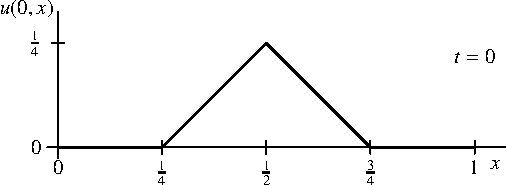
\includegraphics[width=0.8\hsize]{../common/images/burgers-1}
\end{center}
\caption{Anfangsbedingung f"ur die Burgers Gleichung einer idealen
Fl"ussigkeit\label{burgersanfang}}
\end{figure}
In diesem Abschnitt m"ochten wir die Burgers Gleichung f"ur die ideale
Fl"ussigkeit
\[
\frac{\partial}{\partial t}u+\frac{\partial}{\partial x}\left(\frac{u^2}2\right)=0
\]
auf dem Interval $x\in[0,1]$ und f"ur $t>0$
mit der Anfangsbedingung
\[
u(0,x)=\begin{cases}
0\qquad&\text{$x<\frac14$ oder $x>\frac34$}\\
x-\frac14\qquad&\frac14\le x\le \frac12\\
\frac34-x\qquad&\frac12\le x\le \frac34
\end{cases}
\]
l"osen (siehe Abbildung \ref{burgersanfang}).

\begin{figure}
\begin{center}
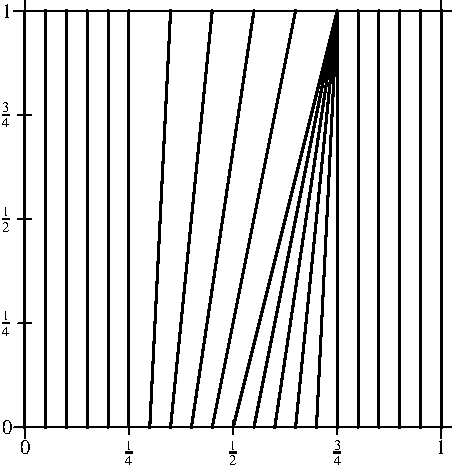
\includegraphics[width=0.8\hsize]{../common/images/burgers-2}
\end{center}
\caption{Niveaulinien (Charakteristiken) der L"osung der Burgers-Gleichung f"ur
die ideale Fl"ussigkeit\label{burgersniveau}}
\end{figure}
Die Differentialgleichung ist von erster Ordnung, in der Form
\[
\partial_tu+u\partial_xu=0
\]
haben wir die zugeh"orige geometrische Theorie in Abschnitt
\ref{pdgl1ordnung} besprochen. Dort wurde darauf hingewiesen,
dass der Vektor 
\[
\begin{pmatrix}
1\\u\\0
\end{pmatrix}
\]
immer an die Fl"ache $u=u(t,x)$ tangential ist. Die L"osungsfl"ache
entsteht dadurch, dass die Anfangsbedingung mit Hilfe dieses Vektors
verschoben wird. 
Der Punkt $(0,x,u(0,x))$ entwickelt sich nach dieser Methode zu
Punkten $(t,x+u(0,x)t, u(0,x))$ der L"osungsfl"ache. Die Kurven
gleichen Funktionswertes bilden also Geraden, deren Steigung im
$x$-$t$-Koordinatensystem $u(0,t)^{-1}$ ist. Die Niveaulinien der
L"osung sehen daher aus wie in der Abbildung \ref{burgersniveau}
dargestellt.
Daraus kann man jetzt auch die L"osungen ablesen. In der Abbildung
\ref{burgerssprung} kann man die Entwicklung der Spitze zu einem
Sprung an der Stelle $x=\frac34$ beobachten.

\begin{figure}
\begin{center}
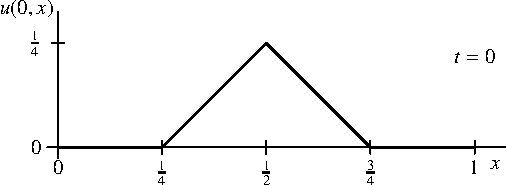
\includegraphics[width=0.8\hsize]{../common/images/burgers-1}
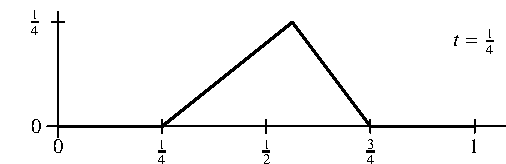
\includegraphics[width=0.8\hsize]{../common/images/burgers-3}
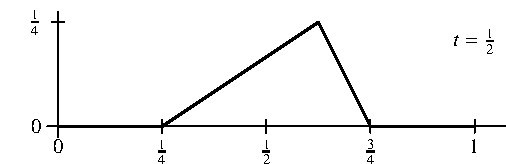
\includegraphics[width=0.8\hsize]{../common/images/burgers-4}
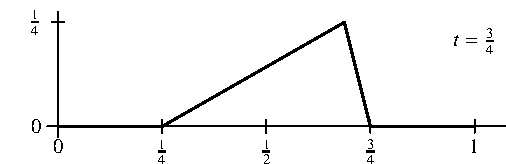
\includegraphics[width=0.8\hsize]{../common/images/burgers-5}
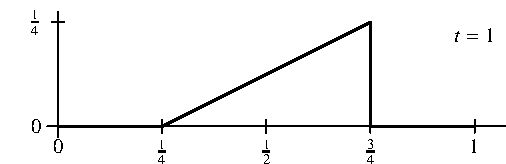
\includegraphics[width=0.8\hsize]{../common/images/burgers-6}
\end{center}
\caption{Entwicklung eines Sprungs in der L"osung der Gleichung von Burgers\label{burgerssprung}}
\end{figure}

Man k"onnte argumentieren, dass die Anfangsbedingung ja bereits nicht differenzierbar
ist, und dass die L"osungen dies ebenfalls nicht sind. Man kann
jedoch eine beliebige glatte Funktion als Anfangsbedingung w"ahlen, welche
innerhalb des Intervals $[\frac14,\frac12]$ monoton von $0$ auf $\frac14$ 
ansteigt, im Punkt $x=\frac12$ den maximalen Wert $\frac14$ annimmt,
und im Interval $[\frac12,\frac34]$ monoton auf $0$ abf"allt.
Das Maximum wird sich entlang der Charakteristiken zum Punkt
$(1,\frac34,\frac14)$ entwicklen. Der Funktionswert $u(0,x)$ im Punkt $(0,x)$
f"ur $x\in[\frac14,\frac12]$ ist derselbe wie im Punkt $(1,x+u(0,x))$.
Der Funktionsgraph $x\mapsto u(1,x)$ hat also die Parameterdarstellung
\[
[{\textstyle\frac14},{\textstyle\frac12}]\to\mathbb R\colon s\mapsto (s+u(0,s),u(0,s))
\]
Diese ist jedenfalls eine glatte Funktion. Andererseits komprimieren
die Charakteristiken das Interval $[\frac12,\frac34]$ auf
den Punkt $(1,\frac34)$ so dass bei $x=\frac34$ wieder ein Sprung entsteht.

